\chapter{Проектирование и реализация сверточной нейронной сети для бинарной классификации изображений на языке Python}
Целью работы является проектирование, реализация и обучение сверточной нейронной сети проводящей дихотомию фотографий различных людей на 2 класса: фотографии с мужчинами и фотографии с женщинами. Для достижения цели был использован язык Python, библиотеки Keras и Tensorflow.
\section{Подготовка к написанию программы}
\subsection{Поиск и подготовка данных для обучения}
Поиск данных для обучения производился в системе организации конкурсов по исследованию данных kaggle. Он содержит множество наборов данных для совершенно различных задач. Для данной работы был выбран набор Gender Classification 200K Images | CelebA. Он содержит около 200000 фотографий лиц различных людей, которые входе работы были разбиты на 3 части:
\begin{enumerate}
    \item [1)] выборка для обучения, около 80000 изображений;
    \item [2)] выборка валидации, около 20000 изображений;
    \item [3)] тестовая выборка, около 100000 изображений.
\end{enumerate}

\subsection{Проектирование архитектуры нейронной сети}
Сверточная нейронная сеть для данной задачи будет состоять из 5 слоев(рисунок \ref{fig:4}):
\begin{enumerate}
    \item [1)] сверточный слой на вход которого будет подаваться цветное растровое изображение в виде тензора размерностью $128 \times 128 \times 3$, с 32 ядрами размерностью $3 \times 3$ и функцией активациии ReLu:
\begin{equation}
\begin{cases}
f(x) = x,  \text{ при } x \geq  0,\\ 
f(x) = 0, \text{ при } x < 0;  
\end{cases}\\[4mm]
\end{equation}
    \item [2)] слой MaxPooling с размером окна $2 \times 2$, который преобразует карту признаков размерностью $128 \times 128 \times 32$ в карту признаков размерностью $64 \times 64 \times 32$;
    \item [3)] входной слой нейронов полносвязной сети, который преобразует карту признаков размерностью $64 \times 64 \times 32$ в вектор, состоящий из $131072$ элементов;
    \item [4)] скрытый слой полносвязной сети в котором 128 нейронов и функция активации ReLu;
    \item [5)] выходной слой, состоящий из 2 нейронов с  функцией активации softmax:
\begin{equation}
f(x) = y_{n} = \frac{e^{v_{n}}}{\sum_{i}^{N}e^{v_{i}}}, n\in N,
\end{equation}
где $v_{n}$ — значение входного сигнала для слоя.
\end{enumerate}


\begin{figure}[!h] 
  \center
  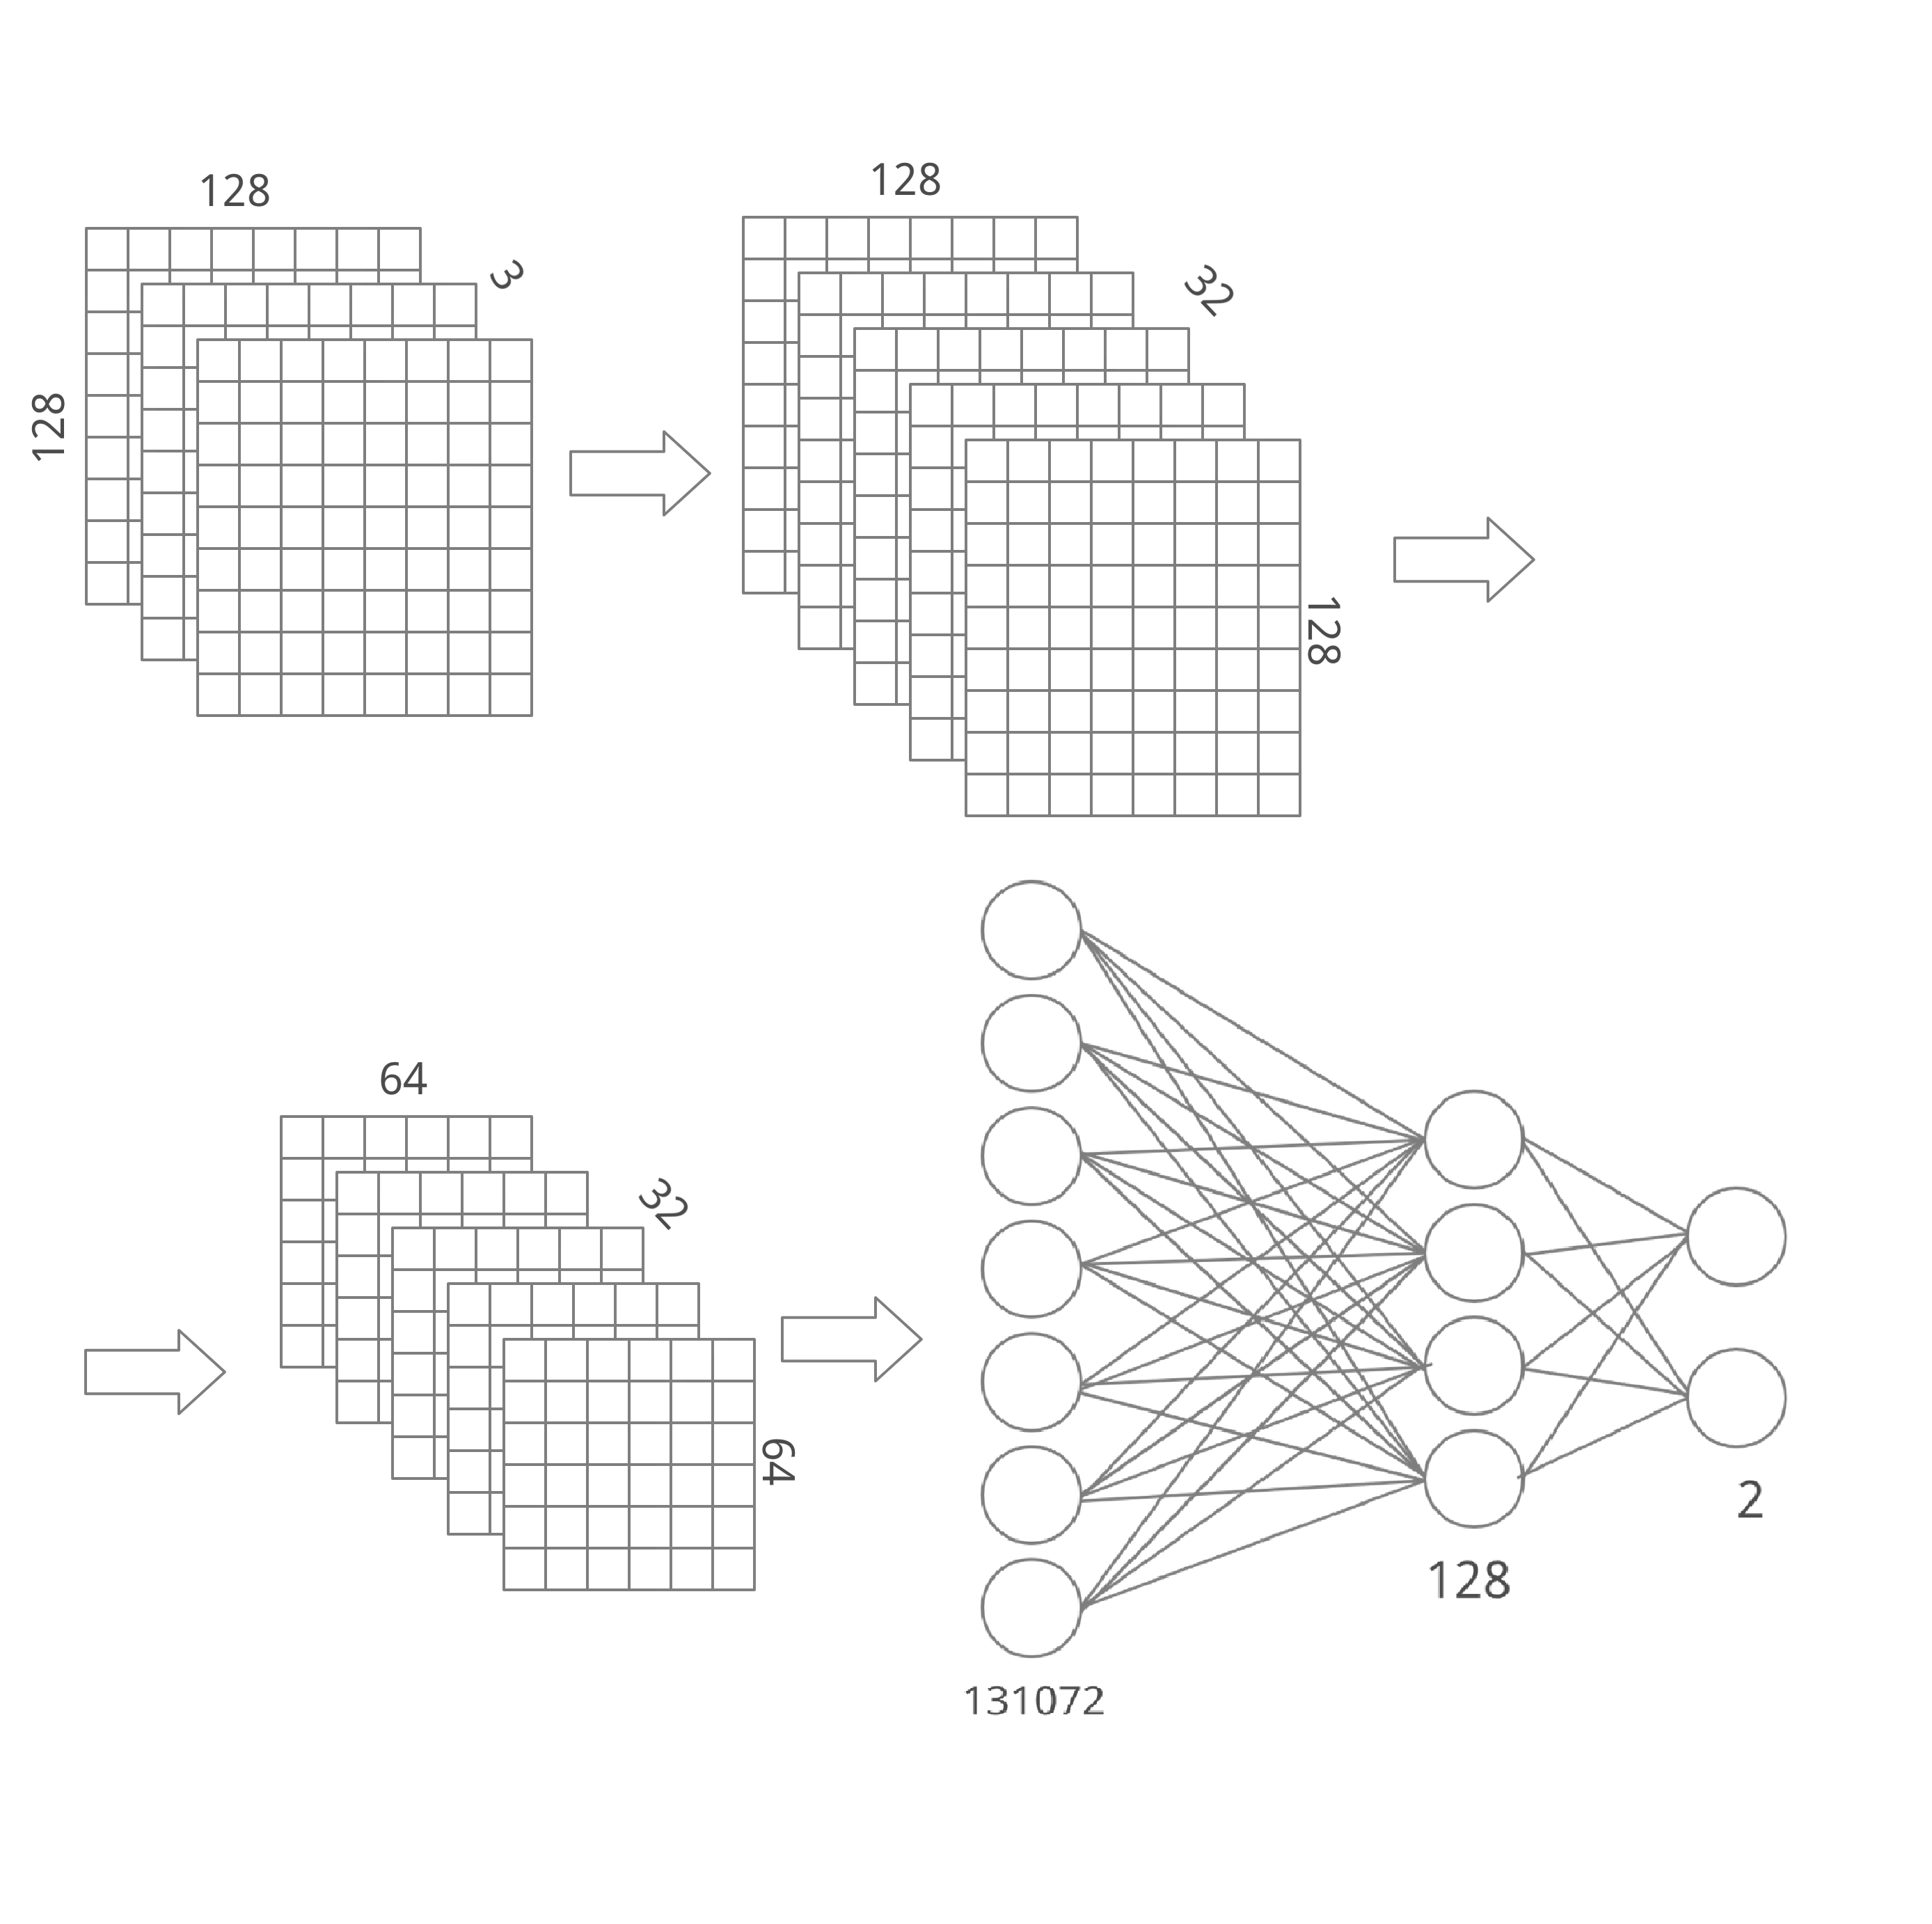
\includegraphics [scale=0.2] {img/project.png}
  \caption{Конечная схема спроектированной модели сверточной нейронной сети} 
  \label{fig:4}  
\end{figure}
\newpage


\section{Реализация модели на языке Python и обучение сети}
Для напсиания программы были использованы библиотеки Keras и Tensorflow. Класс Sequential представляет собой линейный стек слоев. С помощью него можно достаточно просто создать необходимую модель. Он автоматически настраивает все связи между слоями, а также добавляет нейроны смещения. В листенге \ref{ls:1} во входных параметрах передаются 5 слоев:
\begin{enumerate} 
  \item[1)] входной сверточный слой класса Convolution2D, с 32 ядрами размерностью $3 \times 3$, который принимает тензор размерностью $128\times128\times3$ и выдает тензор размерностью $128\times128\times32$, с функцией активации ReLu;
  \item[2)] скрытый слой класса MaxPooling2D, с размером окна $2 \times 2$, который преобразует карту признаков размерностью $128 \times 128 \times 32$ в карту признаков размерностью $64 \times 64 \times 32$;
  \item[3)] скрытый слой класса Flatten, который преобразует карту признаков размерностью $64 \times 64 \times 32$ в вектор, состоящий из $131072$ элементов;
  \item[4)] скрытый слой класса Dense, в котором 128 нейронов, с функцией активации ReLu;
  \item[5)] выходной слой того же класса из 2 нейронов, с функцией активации softmax.
\end{enumerate}

\begin{lstlisting}[caption={Описание модели нейросети},language=python, label={ls:1}]
self.classifier = Sequential(
    [
        Convolution2D(32, (3, 3), input_shape=(self.rez, self.rez, 3), activation='relu'),
        MaxPooling2D(pool_size=(2, 2)),
        Flatten(),
        Dense(128, activation='relu'),
        Dense(2, activation='softmax')
    ]
)
\end{lstlisting}

В листинге \ref{ls:2} указан метод для настройки процесса обучения:

\begin{lstlisting}[caption={Использовние метода compile()},language=python,label={ls:2}]
self.classifier.compile(
    optimizer='adam', 
    loss='sparse_categorical_crossentropy',
    metrics=['accuracy']
)
\end{lstlisting}
Метод compile() на вход принимает 3 параметра:
\begin{enumerate} 
  \item[1)] метод оптимизации алгоритма градиентного спуска. Для данной модели был выбран метод Adam;
  \item[2)] функция ошибки (потерь), он же критерий качества, который программа будет использовать для корректировки весов во время обратного распространения ошибки. Для функции softmax очень хорошо подходит критерий качества категориальная перекрестная энтропия, в общем случае она принимает такой вид:
\begin{equation}
E = - \frac{1}{N}\sum_{m\in N}\sum_{i=1}^{n}t^{(m)}_{i}\log y^{(m)}_{i};
\end{equation}
  \item[3)] метрика, по которой будет оцениваться общая точность модели во время обучения. Метрика <<accuracy>> указывает процент правильных предсказаний.
\end{enumerate}

В листинге \ref{ls:3} данные для обучения загружаются в тензоры с помощью метода flow\_from\_directory класса ImageDataGenerator. Данный класс позволяет также немного изменять входные данные, создавая поворот, приближение и отзеркаливание случайных фотографий для того чтобы не повторяться в различных попытках обучения.
\begin{lstlisting}[caption={Использовние класса ImageDataGenerator и метода flow\_from\_directory},language=python,label={ls:3}]
train_datagen = ImageDataGenerator(
    rescale=1. / 255,
    shear_range=0.2,
    zoom_range=0.2,
    horizontal_flip=True)

val_datagen = ImageDataGenerator(rescale=1. / 255)
test_datagen = ImageDataGenerator(rescale=1. / 255)

training_set = train_datagen.flow_from_directory(
    'C:/Users/Sergey/Desktop/Men-Women/kaggle/input/train_data/',
    target_size=(128, 128),
    batch_size=100,
    class_mode='binary',
    color_mode='rgb')

test_set = test_datagen.flow_from_directory(
    'C:/Users/Sergey/Desktop/Men-Women/kaggle/input/test_data/',
    target_size=(128, 128),
    batch_size=1,
    class_mode='binary',
    color_mode='rgb')

val_set = val_datagen.flow_from_directory(
    'C:/Users/Sergey/Desktop/Men-Women/kaggle/input/val_data/',
    target_size=(128, 128),
    batch_size=1,
    class_mode='binary',
    color_mode='rgb')
\end{lstlisting}

В листинге \ref{ls:4} запускается процесс обучения с помощью метода fit() и сохраняются обученные значения весов в файл classifier.h5 методом save\_weights():
\begin{lstlisting}[caption={Использовние метода fit() и save\_weights()},language=python,label={ls:4}] 
EPOCHS = 20
history = classifier.fit(
    training_set,
    epochs=EPOCHS,
    validation_data=val_set
)
classifier.save_weights('classifier.h5')
\end{lstlisting}

На рисунке \ref{fig:5} изображены графики зависимости точности и ошибок на учебном наборе и на выборке валидации от эпохи обучения. Справедлио заметить, что на выборке валидации процент ошибок после 5 эпохи становится больше, чем на наборе для обучения. Это означает, что алгоритм начинает переобучаться после 5 эпохи. В таком случае стоит остановиться на 5 эпохе обучения и сохранить веса.
\begin{figure}[!h] 
  \center
  \includegraphics [scale=0.5] {img/val_acc_loss20.png}
  \caption{Графики зависимости точности нейронной сети от эпохи обучения} 
  \label{fig:5}  
\end{figure}

Сохранив веса, можно начать проверку точности на тестовой выборке (рисунок \ref{fig:6}), точность составила 95.35\%.
\begin{figure}[!h] 
  \center
  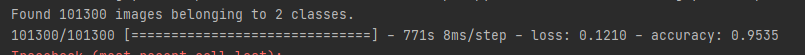
\includegraphics [scale=0.8] {img/testset.png}
  \caption{Данные терминала после начала процесса тестирования} 
  \label{fig:6}  
\end{figure}
\section{Создание интерфейса и тестирование на произвольных фотографиях}
Интефейс программы был написан с помощью библиотеки Tkinter(рисунок \ref{fig:7}). Слева имеется поле для ввода пути к изображению, которое необходимо отнести к одному из классов. Ниже находится кнопка <<Predict>>, которая запускает процесс распознавания. Еще ниже находится область предпросмотра фотографии. В правой части будет выдан ответ male или female, который будет означать кто, по мнению программы, изображен на фотографии --- мужчина или женщина соответсвенно.
\begin{figure}[!h] 
  \center
  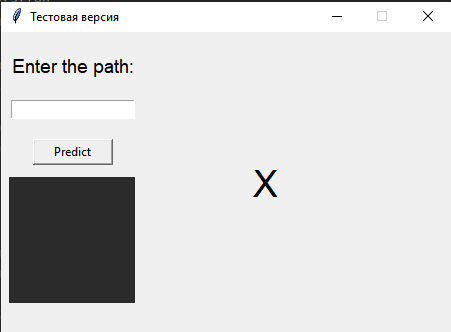
\includegraphics [scale=1.2] {img/interface.png}
  \caption{Интерфейс программы} 
  \label{fig:7}  
\end{figure}

На рисунках \ref{fig:8}, \ref{fig:9}, \ref{fig:10}, \ref{fig:11}, \ref{fig:12}, \ref{fig:13} приведено тестирование на различных фотографиях мужчин и женщин. 
\begin{figure}[!h] 
  \center
  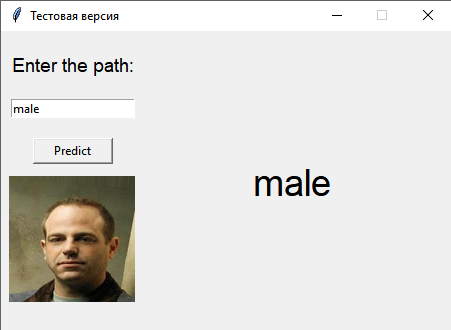
\includegraphics [scale=1.2] {img/testmale1.png}
  \caption{Тестирование фотографии мужчины} 
  \label{fig:8}  
\end{figure}

\begin{figure}[!h] 
  \center
  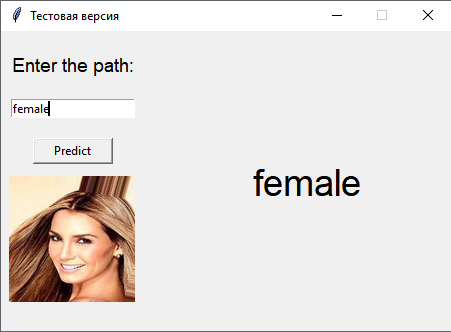
\includegraphics [scale=1.2] {img/testfemale1.png}
  \caption{Тестирование фотографии женщины} 
  \label{fig:9}  
\end{figure}

\begin{figure}[!h] 
  \center
  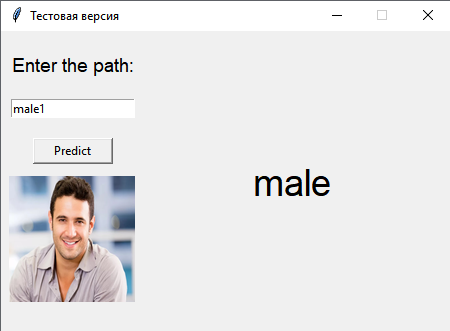
\includegraphics [scale=1.2] {img/testmale2.png}
  \caption{Тестирование фотографии мужчины} 
  \label{fig:10}  
\end{figure}

\begin{figure}[!h] 
  \center
  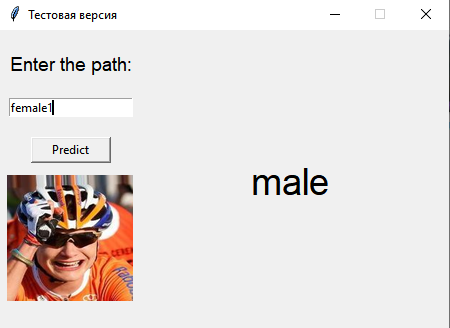
\includegraphics [scale=1.2] {img/testfemale2.png}
  \caption{Тестирование фотографии женщины} 
  \label{fig:11}  
\end{figure}
\begin{figure}[!h] 
  \center
  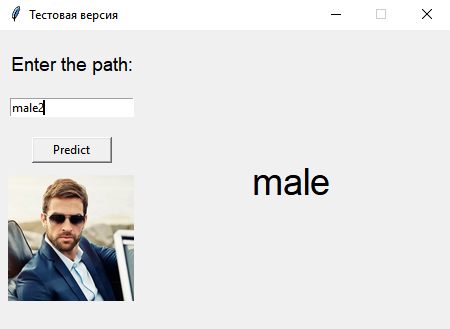
\includegraphics [scale=1.2] {img/testmale3.png}
  \caption{Тестирование фотографии мужчины} 
  \label{fig:12}  
\end{figure}

\begin{figure}[!h] 
  \center
  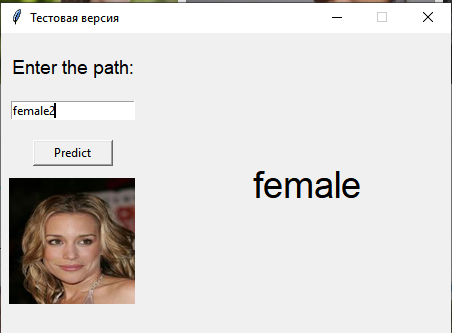
\includegraphics [scale=1.2] {img/testfemale3.png}
  \caption{Тестирование фотографии женщины} 
  \label{fig:13}  
\end{figure}
\newpage
На произвольных фотографиях программа справляется довольно хорошо, допуская ошибки только в самых сложных примерах, в которых могут быть перекрыты части лица одеждой, снаряжением или окружением.(рисунок \ref{fig:11}).
